\documentclass{article}

\usepackage{graphicx}
\usepackage{rotating}
\usepackage{amsmath}
\usepackage{mathtools}
\usepackage{nccmath}
\usepackage{tikz}
\usepackage{fancyhdr}
\usepackage{listings}
\usepackage{xcolor}
\usepackage{color}
\usepackage{amsfonts}
\usepackage{textcomp}
\usepackage{float}
\usepackage[sorting=none]{biblatex}
\usepackage[margin=1in]{geometry}
\usepackage[font={small,it}]{caption}
\usepackage{placeins}
\usepackage{xepersian}



%\DeclareMathOperator*{\btie}{\bowtie}
\addbibresource{bibliography.bib}
\settextfont[Scale=1.2]{B-NAZANIN.TTF}
\setlatintextfont[Scale=1]{Times New Roman}
\renewcommand{\baselinestretch}{1.5}
\pagestyle{fancy}
\fancyhf{}
\rhead{تکلیف دوم درس هوش مصنوعی (بخش تئوری)}
\lhead{\thepage}
\rfoot{علیرضا ابره فروش}
\lfoot{9816603}
\renewcommand{\headrulewidth}{1pt}
\renewcommand{\footrulewidth}{1pt}
%%%%%%%%%%
\lstset
{
    language=[latex]tex,
    basicstyle=\ttfamily,
    commentstyle=\color{black},
    columns=fullflexible,
    keepspaces=true,
    upquote=true,
    showstringspaces=false,
    morestring=[s]\\\%,
    stringstyle=\color{black},
}
%%%%%%%%%%
%beginMatlab
\definecolor{mygreen}{RGB}{28,172,0} % color values Red, Green, Blue
\definecolor{mylilas}{RGB}{170,55,241}
%endMatlab
\begin{document}
%beginMatlab
\lstset{language=Matlab,%
    %basicstyle=\color{red},
    breaklines=true,%
    morekeywords={matlab2tikz},
    keywordstyle=\color{blue},%
    morekeywords=[2]{1}, keywordstyle=[2]{\color{black}},
    identifierstyle=\color{black},%
    stringstyle=\color{mylilas},
    commentstyle=\color{mygreen},%
    showstringspaces=false,%without this there will be a symbol in the places where there is a space
    numbers=left,%
    numberstyle={\tiny \color{black}},% size of the numbers
    numbersep=9pt, % this defines how far the numbers are from the text
    emph=[1]{for,end,break},emphstyle=[1]\color{red}, %some words to emphasise
    %emph=[2]{word1,word2}, emphstyle=[2]{style},    
}
%endMatlab
\begin{titlepage}
\begin{center}

\includegraphics[width=0.4\textwidth]{figures/IUT Logo.png}\\
        
\LARGE
\textbf{دانشگاه صنعتی اصفهان}\\
\textbf{دانشکده مهندسی برق و کامپیوتر}\\
        
\vfill
        
\huge
\textbf{عنوان: تکلیف چهارم درس ریزپردازنده}\\
        
\vfill
        
\LARGE
\textbf{نام و نام خانوادگی: علیرضا ابره فروش}\\
\textbf{شماره دانشجویی: 9816603}\\
\textbf{نیم\,سال تحصیلی: پاییز 1400}\\
\textbf{مدرّس: دکتر عارف کریمی افشار}\\
\end{center}
\end{titlepage}


%\tableofcontents
\newpage


\section{نوید زندانی}
\subsection{قیدهای \lr{binary} و \lr{unary}}
\begin{fleqn}
\begin{equation}
\begin{aligned}
\forall i\in \left\{ 1,2,3,4,5,6 \right\}\:\:\:\:\:\: Y_{i} = \begin{cases}
    0 & X_{i} = \text{زندان} \\
    1 & X_{i} = \text{خروج} \\
    2 & X_{i} = \text{چاه}
\end{cases}
\end{aligned}
\end{equation}
\end{fleqn}


\begin{fleqn}
\begin{equation}
\begin{aligned}
C_{1} = \left\langle \left( X_{1},\: X_{2} \right),\: \max\left\{ Y_{1},\: Y_{2} \right\} = 1 \right\rangle \\
C_{2} = \left\langle \left( X_{2},\: X_{3} \right),\: \max\left\{ Y_{2},\: Y_{3} \right\} = 1 \right\rangle \\
C_{3} = \left\langle \left( X_{3},\: X_{4} \right),\: \max\left\{ Y_{3},\: Y_{4} \right\} = 2 \right\rangle \\
C_{4} = \left\langle \left( X_{4},\: X_{5} \right),\: \max\left\{ Y_{4},\: Y_{5} \right\} = 2 \right\rangle \\
C_{5} = \left\langle \left( X_{5},\: X_{6} \right),\: \max\left\{ Y_{5},\: Y_{6} \right\} = 2 \right\rangle \\
C_{6} = \left\langle \left( X_{6},\: X_{1} \right),\: \max\left\{ Y_{6},\: Y_{1} \right\} = 2 \right\rangle
\end{aligned}
\end{equation}

\begin{equation}
\begin{aligned}
C_{7} = \left\langle \left( X_{1},\: X_{2} \right),\: Y_{1} \times Y_{2} \neq 1 \right\rangle \\
C_{8} = \left\langle \left( X_{2},\: X_{3} \right),\: Y_{2} \times Y_{3} \neq 1 \right\rangle \\
C_{9} = \left\langle \left( X_{3},\: X_{4} \right),\: Y_{3} \times Y_{4} \neq 1 \right\rangle \\
C_{10} = \left\langle \left( X_{4},\: X_{5} \right),\: Y_{4} \times Y_{5} \neq 1 \right\rangle \\
C_{11} = \left\langle \left( X_{5},\: X_{6} \right),\: Y_{5} \times Y_{6} \neq 1 \right\rangle \\
C_{12} = \left\langle \left( X_{6},\: X_{1} \right),\: Y_{6} \times Y_{1} \neq 1 \right\rangle
\end{aligned}
\end{equation}
\end{fleqn}







\subsection{}
\subsection{}
\subsection{}
\subsection{}
\subsection{}



\section{مسئله سه رنگ}
هر \lr{Candidate solution} در این مسئله را می‌توان نظیر یک رشته به طول $n$ از اعداد موجود در مجموعه‌ی $G_{l}$ در نظر گرفت (نمایش اعداد صحیح) به طوری که $i$ بودن کاراکترِ $m$ام به معنی قرار گرفتن جسمِ $m$ام در ستونِ $i$ام است. همچنین مجموعه‌ی همسایگی نظیر یک \lr{Candidate solution} را می‌توان به شکل مجموعه‌ی همه‌ی رشته‌هایی که با رشته مذکور دقیقا در یک کاراکتر اختلاف دارند، تعریف کرد.



\section{\lr{consistency}}
هر \lr{Candidate solution} در این مسئله را می‌توان به یک جایگشت از اعداد 1 تا $n$ نظیر کرد به طوری که $i$ بودنِ جایگاه $m$ام به معنی نگاشتِ مرکز رفاهیِ $i$ به مکانِ $m$ است. مجموعه‌ی شامل همه‌ی جایگشت‌های اعداد 1 تا $n$ را با $P_{n}$ نشان می‌دهیم.
به ازای هر جایگشت در $P_{n}$، تابعِ $\phi$ را تعریف می‌کنیم نگاشت از مرکز رفاهی به مکان نظیرِ آن مرکز رفاهی در آن جایگشت. همچنین مجموعه‌ی 
$
S_{n}
$
را تعریف می‌کنیم مجموعه‌ی همه‌ی $\phi$ها. 
 تابعِ 
$
d(i, j)
$
فاصله‌ی بین دو مکان و تابعِ 
$
f(i, j)
$
جریان بین دو مرکز رفاهی را برمی‌گرداند. در واقع کمینه‌سازیِ تابع هدف به شکل زیر شکل می‌گیرد:
\begin{latin}
$
min_{\phi \in S_{n}}(\sum_{i=1}^{n}\sum_{j=1}^{n} f(i, j)\times d(\phi(i), \phi(j)))
$
\end{latin}
در جایگشت همسایگی‌ها به شکل \lr{2-swap} می‌توانند تعریف شوند که در این صورت تابعِ هدف نظیر همسایه‌ی یک \lr{Candidate solution} تنها با تغییر
$f(i, j)\times d(\phi(i), \phi(j))$
به ازای $i$ و $j$های جایگزین شده میسر است و لازم به محاسبه مجدد همه‌ی عبارات نیست.


\section{مدل‌سازی}
\subsection{}
شهرها را با $C_{i}$ و جمعیت آن‌ها را با $p_{i}$ نمایش می‌دهیم. به ازای هر جاده بین دو شهر $C_{i}$ و $C_{j}$ قیدِ
\begin{equation}
\left| p_{i} - p_{j} \right| \ge 2000
\end{equation}
را داریم. همچنین برای براي جلوگيري از به وجود آمدن كلان‌شهر قیدِ
\begin{equation}
\max_{i}\left\{ p_{i} \right\} \le 3\min_{j}\left\{ p_{j} \right\}
\end{equation}
را داریم.

\subsection{}








\section{برنامه‌ریزی کلاس‌ها}
\subsection{}
مسئله را به شکل \lr{CSP}ِ زیر مدل می‌کنیم: \\
$
X_{1} = \text{استاد کلاس 1} \\
X_{2} = \text{استاد کلاس 2} \\
X_{3} = \text{استاد کلاس 3} \\
X_{4} = \text{استاد کلاس 4} \\
X_{5} = \text{استاد کلاس 5} \\
\\
D_{1} = \left\{ \text{پ} \right\} \\
D_{2} = \left\{ \text{ب}, \: \text{پ} \right\} \\
D_{3} = \left\{ \text{الف}, \: \text{ب}, \: \text{پ} \right\} \\
D_{4} = \left\{ \text{الف}, \: \text{ب}, \: \text{پ} \right\} \\
D_{5} = \left\{ \text{ب}, \: \text{پ} \right\} \\
\\
C_{1} = \left\langle \left( X_{1},\: X_{2} \right),\: X_{1} \neq X_{2} \right\rangle \\
C_{2} = \left\langle \left( X_{2},\: X_{3} \right),\: X_{2} \neq X_{3} \right\rangle \\
C_{3} = \left\langle \left( X_{3},\: X_{4} \right),\: X_{3} \neq X_{4} \right\rangle \\
C_{4} = \left\langle \left( X_{4},\: X_{2} \right),\: X_{4} \neq X_{2} \right\rangle \\
C_{5} = \left\langle \left( X_{4},\: X_{5} \right),\: X_{4} \neq X_{5} \right\rangle \\
C_{6} = \left\langle \left( X_{5},\: X_{3} \right),\: X_{5} \neq X_{3} \right\rangle \\
\\
\\
X = \left\{ X_{1},\: X_{2},\: X_{3},\: X_{4},\: X_{5} \right\} \\
D = \left\{ D_{1},\: D_{2},\: D_{3},\: D_{4},\: D_{5} \right\} \\
C = \left\{ C_{1},\: C_{2},\: C_{3},\: C_{4},\: C_{5},\: C_{6} \right\} \\
$

\subsection{}
%graph
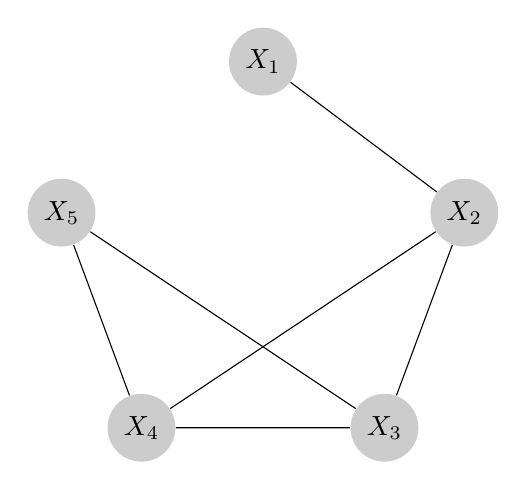
\begin{tikzpicture}
  [scale=.8,auto=left,every node/.style={circle,fill=black!20}]
  \node (n1) at (0,3.3125) {$X_{1}$};
  \node (n2) at (3.197,0.91475)  {$X_{2}$};
  \node (n3) at (1.9285,-2.5)  {$X_{3}$};
  \node (n4) at (-1.9285,-2.5) {$X_{4}$};
  \node (n5) at (-3.197,0.91475)  {$X_{5}$};

  \foreach \from/\to in {n1/n2,n2/n3,n2/n4,n3/n4,n3/n5,n4/n5}
    \draw (\from) -- (\to);

\end{tikzpicture}
%graph

\section{\lr{Puzzle Cryptarithmetic}}


%%%%%%%%%%%%%%%%%%%%%%%%%%%%%%%%%%%
%%%%%%%%%%%%%%%%%%%%%%%%%%%%%%%%%%%
%%%%%%%%%%%%%%%%%%%%%%%%%%%%%%%%%%%

\section*{منابع}
\renewcommand{\section}[2]{}%
\begin{thebibliography}{99} % assumes less than 100 references
%چنانچه مرجع فارسی نیز داشته باشید باید دستور فوق را فعال کنید و مراجع فارسی خود را بعد از این دستور وارد کنید


\begin{LTRitems}

\resetlatinfont

\bibitem{b1}
\end{LTRitems}

\end{thebibliography}


\end{document}
